\documentclass[journal]{IEEEtran}
% Target: IEEE Internet of Things Journal, at most 8 published pages, aim 7.5.
\usepackage{amsmath,amssymb}
\usepackage{graphicx}
\usepackage{booktabs}
\usepackage{cite}
\usepackage{url}
\usepackage{tikz}
\usetikzlibrary{arrows.meta,positioning}


\begin{document}

\title{Network-Side Doppler Mitigation for\\ Direct-to-Satellite LoRaWAN Using\\ Gateway Reception Statistics}

\author{Mehran~M.~Mamonai%
\thanks{Manuscript draft, November 2026.}%
\thanks{M.~M.~Mamonai is with the Department of Telecommunication Engineering, Mehran University of Engineering and Technology, Jamshoro, Pakistan (e-mail: mehran.mamonai@faculty.muet.edu.pk).}}

\markboth{IEEE Internet of Things Journal (draft)}{Network-Side Doppler Mitigation for Direct-to-Satellite LoRaWAN Using Gateway Reception Statistics}

\maketitle

\begin{abstract}
Direct-to-satellite LoRaWAN lets unmodified Internet of Things devices reach a low Earth orbit gateway, but at 868~MHz the Doppler rate near zenith can exceed what a spreading factor (SF)~12 receiver tolerates. Devices that choose their SF from the link budget alone then lose packets at high elevation. We ask whether a controller at the satellite gateway, using only the reception statistics the network already has, can remove part of this loss without harming delivery. We implement a per-pass control loop in a full-stack ns-3 LoRaWAN model of a 560~km orbit with 3GPP TR~38.811 channels, and evaluate it under three collision models and four literature-based readings of the unmeasured SF12 Doppler-rate limit. The controller learns one elevation above which SF12 is withheld and distributes it in Class~B beacons. It converges within two passes, never lowers delivery in any of 192 scenarios, and clearly lowers the Doppler-loss share in 24 of the 34 scenarios where the loss occurs, for example from 13.0\% to 11.2\%. An oracle that knows the true limit still delivers 1.3 to 1.5 times as much. Updating every device instantly closes only 1\% of that gap, so beacon reach does not explain it. The coarse threshold does, because the Doppler rate at a given elevation depends on how close the pass comes to zenith. We also report a negative result: thinning the offered load from gateway counters never avoided harm under measured collision thresholds.
\end{abstract}

\begin{IEEEkeywords}
LoRaWAN, direct-to-satellite IoT, low Earth orbit, Doppler, spreading factor, network control, ns-3.
\end{IEEEkeywords}

\section{Introduction}
\IEEEPARstart{L}{oRaWAN} devices can reach a gateway carried by a low Earth orbit (LEO) satellite without any change to their radio, which makes direct-to-satellite IoT attractive for sensors far from terrestrial coverage~\cite{alvarez2022,asadullah2024}. The link is long and short-lived. A satellite at 560~km stays in view for a few minutes per pass, and devices often need the slowest data rate, SF12, to close the link budget.

At high elevation, SF12 runs into a second limit. The Doppler shift changes fastest when the satellite passes overhead, and LoRa demodulation tolerates only a bounded Doppler \emph{rate} at long symbol times. Flight tests at 436.7~MHz saw no Doppler loss at SF12 and 125~kHz up to about 143~Hz/s~\cite{zadorozhny2022}, and laboratory tests put the SF12 limit near 144~Hz/s~\cite{doroshkin2019}. At 868~MHz the peak rate on a 560~km orbit roughly doubles to about 273~Hz/s, so SF12 packets sent near zenith may be lost. Whether they are depends on a limit that has not been measured at 868~MHz: an emulation study at that frequency reports loss already near 93~Hz/s~\cite{colombo2022}, while reading the laboratory limit as 0.33~ppm/s instead of a fixed rate leaves no loss at all~\cite{doroshkin2019}.

A device sending unconfirmed uplinks has no way to notice this loss. The gateway is better placed. It records the SF, timing and signal strength of every packet it receives~\cite{sx1301}, so a shortfall of SF12 receptions at high elevation shows up in its counters. This points to a network-side controller in the style of the O-RAN non-real-time loop~\cite{tarchi2026}, which reads the counters after each pass and sends new settings to devices in the next Class~B beacon~\cite{lorawanL2}.

This paper tests that idea in a full-stack simulation. Its contributions are:
\begin{enumerate}
\item A per-pass control loop for direct-to-satellite LoRaWAN, implemented in ns-3, that learns an SF12 elevation cut-off from aggregated reception counts and distributes it in Class~B beacons. It needs no device-side computation and no ground truth about Doppler or losses.
\item An evaluation across 192 scenarios, three collision models (one analytical, one measured, one measured with receiver locking~\cite{goursaud2015,croce2018,bor2016}) and four readings of the SF12 Doppler-rate limit, with pass criteria fixed before each run. The controller never lowers delivery, and clearly lowers Doppler loss in 24 of the 34 scenarios where the loss occurs.
\item A diagnosis of the remaining gap to an oracle. Delivering settings to every device instantly closes only 1\% of it; the rest comes from using one elevation threshold for all pass geometries.
\item A negative result: under measured collision thresholds, no rule that thins load from gateway counters avoided harm.
\end{enumerate}

Section~\ref{sec:related} reviews related work. Section~\ref{sec:model} describes the system model and Section~\ref{sec:controller} the controller. Section~\ref{sec:method} gives the evaluation method, Section~\ref{sec:results} the results, and Section~\ref{sec:discussion} the limitations.

\section{Related Work}\label{sec:related}
\emph{Uplink policies for direct-to-satellite LoRa.} Alvarez et al.~\cite{alvarez2022} compare uplink policies that use the satellite trajectory: transmitting only during the pass, choosing the lowest SF that closes the link at the current distance, and skipping transmissions with a probability carried in a beacon. Their trajectory-based SF choice is our link-only baseline; their policies do not model Doppler limits. Tondo et al.~\cite{tondo2024} schedule multi-channel access and omit Doppler, citing flight tests that saw little impact.

\emph{Doppler.} Asad Ullah et al.~\cite{asadullah2024} derive static and dynamic Doppler limits for LoRa and report losses at high elevation. Flight tests at 436.7~MHz contradict their dynamic limit at SF12 and 125~kHz, measuring no Doppler loss up to about 143~Hz/s~\cite{zadorozhny2022}, consistent with laboratory tests~\cite{doroshkin2019}. The only 868~MHz SF12 data we found is an SDR emulation~\cite{colombo2022}. Maleki et al.~\cite{maleki2026} use reinforcement learning to choose SF, bandwidth, coding rate and timing per device with a Doppler loss model; their evaluation is analytical and assumes coordination is available.

\emph{Load control.} Herreria-Alonso et al.~\cite{herreria2023} adapt each device's transmit probability from its own success rate. Vogelgesang et al.~\cite{vogelgesang2021} broadcast a transmit probability in Class~B beacons that maximizes expected successes when the number of contending devices is known, and leave its estimation open. FSMA~\cite{fsma2026} lets the gateway signal a free channel so that weak devices filter themselves.

Unlike these studies, our controller acts once per pass and uses network-side observations only. We evaluate it on a full LoRaWAN stack with measured collision thresholds and report each result across the range of Doppler limits that the literature allows.

\section{System Model}\label{sec:model}

Fig.~\ref{fig:arch} shows the system. Static devices in a remote area send uplinks to a LoRaWAN gateway carried by a low Earth orbit satellite. The network server bins the receptions of each pass by elevation, a network-side controller turns these counts into an SF12 elevation cut-off $\theta$, and the satellite sends $\theta$ to the devices in Class~B beacons during the next pass. The rest of this section describes each part and the assumptions behind it.

\begin{figure*}[t]
\centering
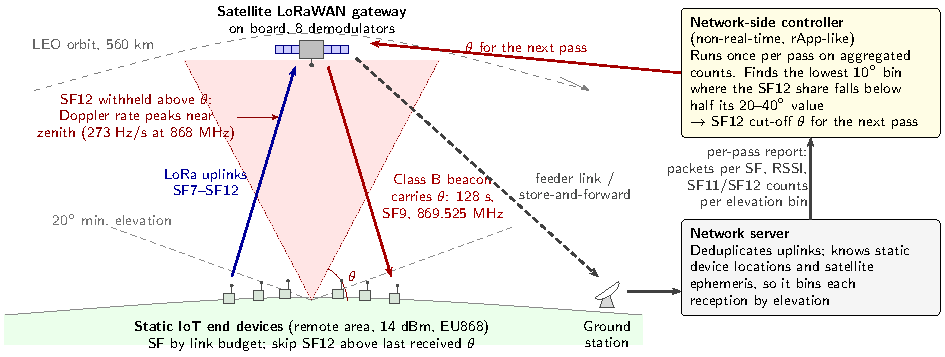
\includegraphics[width=\textwidth]{figs/fig_architecture.pdf}
\caption{\textbf{System architecture.} Devices choose their SF from the link budget and skip SF12 above the last cut-off $\theta$ they received. Near zenith the Doppler rate is highest, so SF12 packets there are lost under the Doppler limits of Section~\ref{sec:model}-B. After each pass the network server reports aggregated reception counts, and the controller returns $\theta$, which reaches devices in Class~B beacons. The feeder link between satellite and ground is shown for completeness and is not modeled; in the simulation the per-pass report reaches the controller directly. The cone angle is schematic.}
\label{fig:arch}
\end{figure*}

\subsection{Orbit, Link and Channel}
A satellite in a 560~km circular orbit~\cite{asadullah2024} carries a LoRaWAN gateway. Devices on the ground send 32-byte frames at 14~dBm on the three default EU868 channels at 125~kHz, one attempt per 60~s and at most 1\% duty cycle~\cite{traspadini2025,casals2017,lorawanRP}. Table~\ref{tab:params} lists the parameters. The total antenna gain is 5 or 10~dBi~\cite{traspadini2025}. Devices transmit only above 20$^\circ$ elevation~\cite{tr38811,santana2026}.

The channel follows the rural model of 3GPP TR~38.811~\cite{tr38811}: elevation-dependent line-of-sight probability, shadow fading and clutter loss, and Rician fading in line of sight. We apply the S-band values at 868~MHz, as Sant'Ana et al.~\cite{santana2026} do; this is an extrapolation. Ionospheric scintillation adds 7.69~dB at low latitude (up to 20$^\circ$) and nothing at mid-latitude~\cite{tr38811}. Gateway sensitivity runs from $-123$~dBm at SF7 to $-137$~dBm at SF12~\cite{santana2026,herreria2023}.

\begin{table}[t]
\centering
\caption{Simulation parameters}\label{tab:params}
\begin{tabular}{@{}ll@{}}
\toprule
Parameter & Value \\
\midrule
Orbit & 560 km circular \\
Carrier, bandwidth & 868.1 MHz, 125 kHz \\
Transmit power, payload & 14 dBm, 32 bytes (PHY) \\
Attempt period, duty cycle & 60 s, 1\% \\
Total antenna gain & 5 or 10 dBi \\
Minimum elevation & 20$^\circ$ \\
Channel & TR 38.811 rural \\
Scintillation & 7.69 dB (low lat.), 0 dB (mid lat.) \\
Gateway sensitivity, SF7--SF12 & $-123$ to $-137$ dBm \\
Gateway demodulators & 8 \\
Beacon & 128 s, SF9, 869.525 MHz, 500 mW e.r.p. \\
Devices & 100, 500, 2000, 5000 \\
Passes per run & 20 \\
\bottomrule
\end{tabular}
\end{table}

\subsection{Doppler Limits}
For a device at slant range $\rho(t)$ from the satellite, the Doppler shift and its rate are
\begin{equation}\label{eq:doppler}
f_D(t)=-\frac{f_c}{c}\,\dot\rho(t),\qquad \dot f_D(t)=-\frac{f_c}{c}\,\ddot\rho(t),
\end{equation}
with carrier frequency $f_c$ and speed of light $c$~\cite{asadullah2024}. The shift is largest at low elevation and the rate is largest at the point of closest approach, so the two limits bite at opposite ends of a pass. Both scale with $f_c$. For our 560~km orbit the peak rate on a zenith pass is 137~Hz/s at 436.7~MHz, within 5\% of the 143--144~Hz/s reported for the flight orbit~\cite{zadorozhny2022,asadullah2024}, and 273~Hz/s at 868.1~MHz. The largest shift, at 20$^\circ$ elevation, is 19.0~kHz at 868.1~MHz.

For each packet the simulator evaluates \eqref{eq:doppler} over the packet's time on air. A packet is lost if the shift exceeds the static limit of 25\% of the bandwidth~\cite{asadullah2024,zadorozhny2022}, or if the rate exceeds the dynamic limit for its SF. With 31.25~kHz at 125~kHz bandwidth, the static limit does not bind above 20$^\circ$ in our scenarios, so all Doppler losses are rate losses. SF11 and SF12 use low data rate optimization, as the radio requires at 125~kHz~\cite{sx1276}.

The SF12 dynamic limit at 868~MHz has not been measured, so we carry four readings:
\begin{itemize}
\item \textbf{R1}: 144~Hz/s, the laboratory limit at 434~MHz~\cite{doroshkin2019}, applied as a fixed rate.
\item \textbf{R2}: 93~Hz/s, the rate at which the 868~MHz emulation first shows loss~\cite{colombo2022}.
\item \textbf{R3}: 0.33~ppm/s, the same laboratory limit read in relative terms. At 868~MHz this is about 286~Hz/s, above the 273~Hz/s peak, so SF12 has no Doppler loss.
\item \textbf{R4}: R1 without any dynamic limit at SF10.
\end{itemize}
Under R1--R3, SF10 (which runs without low data rate optimization) keeps the analytical limit of~\cite{asadullah2024}. No flight or laboratory data exists for it, so R4 removes it.

\subsection{Collision Models}
Collision outcomes at high load depend strongly on the capture model, and measured thresholds differ from the ns-3 default by more than 10~dB~\cite{croce2018}. We therefore run every scenario under three models:
\begin{itemize}
\item \textbf{C1}: the Goursaud table~\cite{goursaud2015}, the ns-3 default; a same-SF packet survives if it is 6~dB stronger.
\item \textbf{C2}: thresholds measured on an SX1272~\cite{croce2018}; same SF needs about 1~dB, and cross-SF interferers are tolerated only 8 to 25~dB stronger.
\item \textbf{C3}: C2 plus receiver locking~\cite{bor2016,rahmadhani2018}; a packet is lost if a detectable same-SF packet on the same channel started more than three symbols earlier and is still on the air.
\end{itemize}
At 5000 devices, C2 delivers 1.57 to 2.07 times as many packets as C1, so high-load results are reported as ranges across models.

\subsection{Simulator}
We extend the ns-3 LoRaWAN module~\cite{ns3lorawan} with the orbit, channel and Doppler models above, a writable gateway sensitivity table, uplink-only delivery to the gateway, and the C2 and C3 interference rules. The controller runs as a separate process that exchanges one JSON line per pass with the simulator. With a controller that returns constant settings, all 256 test runs reproduce the uncontrolled runs exactly. The simulator extensions, the controller, the run scripts and the data behind every figure and table are available at \url{https://github.com/mehranmamonai/lora-ntn}.

\section{Network-Side SF12 Control}\label{sec:controller}

\subsection{Control Loop}
Fig.~\ref{fig:loop} shows the loop. After each pass the network reports what a LoRaWAN gateway can observe~\cite{sx1301}: received packets per SF, distinct devices heard, mean and minimum received power, and the count of SF11 and SF12 receptions in seven 10$^\circ$ elevation bins from 20$^\circ$ to 90$^\circ$. Binning by elevation assumes the network server knows each static device's location, as is common for fixed sensors, and the satellite's own position; the controller receives only the aggregated counts. It returns the settings for the next pass. It never sees the true Doppler or losses at the device.

\begin{figure}[t]
\centering
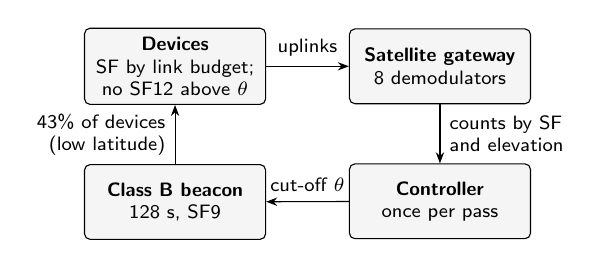
\begin{tikzpicture}[font=\sffamily\scriptsize, >={Stealth[length=4pt]},
  box/.style={draw, rounded corners=2pt, align=center, minimum width=2.3cm, minimum height=0.95cm, fill=black!4}]
\node[box] (dev) {\textbf{Devices}\\ SF by link budget;\\ no SF12 above $\theta$};
\node[box, right=1.05cm of dev] (gw) {\textbf{Satellite gateway}\\ 8 demodulators};
\node[box, below=0.75cm of gw] (ctl) {\textbf{Controller}\\ once per pass};
\node[box, below=0.75cm of dev] (bcn) {\textbf{Class B beacon}\\ 128 s, SF9};
\draw[->] (dev) -- node[above]{uplinks} (gw);
\draw[->] (gw) -- node[right, align=left]{counts by SF\\ and elevation} (ctl);
\draw[->] (ctl) -- node[above]{cut-off $\theta$} (bcn);
\draw[->] (bcn) -- node[left, align=right]{43\% of devices\\ (low latitude)} (dev);
\end{tikzpicture}
\caption{\textbf{Only aggregated network observations enter the controller.} After each pass the gateway reports reception counts; the controller returns the SF12 cut-off $\theta$, which reaches a device only through a beacon it receives.}
\label{fig:loop}
\end{figure}

\subsection{Cut-Off Rule}
Let $n^{(11)}_b$ and $n^{(12)}_b$ be the SF11 and SF12 receptions accumulated in elevation bin $b\in\{0,\dots,6\}$, where bin $b$ covers $[20+10b,\,30+10b)$ degrees, and let
\begin{equation}
s_b=\frac{n^{(12)}_b}{n^{(11)}_b+n^{(12)}_b},\qquad
s_{\mathrm{ref}}=\frac{\sum_{b=0}^{1}n^{(12)}_b}{\sum_{b=0}^{1}\bigl(n^{(11)}_b+n^{(12)}_b\bigr)}
\end{equation}
be the SF12 share in bin $b$ and in the reference band from 20$^\circ$ to 40$^\circ$, where Doppler rates are low. The cut-off is
\begin{equation}\label{eq:cutoff}
\theta=20^\circ+10^\circ\cdot\min\{\,b\ge2:\ n^{(11)}_b+n^{(12)}_b\ge5,\ s_b<\tfrac12 s_{\mathrm{ref}}\,\},
\end{equation}
or $90^\circ$ if no bin qualifies or the reference band holds fewer than five packets. The rule detects the elevation above which SF12 packets stop arriving in the proportion seen at low elevation. A device that would choose SF12 above $\theta$ skips that attempt, except with probability 0.1, which keeps SF12 observations coming from above the cut-off.

\subsection{Setting Distribution}
The satellite sends a Class~B beacon every 128~s at SF9 on 869.525~MHz in implicit mode with a 10-symbol preamble~\cite{lorawanL2,lorawanRP}, carrying the current cut-off. Its time on air is 152.6~ms, a 0.12\% duty cycle. We assume 500~mW e.r.p., the limit for the 869.4--869.65~MHz short-range band~\cite{erc7003}; a satellite downlink would be licensed separately. A device keeps its last received setting. At low latitude, 43\% of devices hear at least one beacon per run; at mid-latitude all do.

\subsection{Baselines}
\emph{Link-only} chooses the lowest SF whose link budget closes at the current distance, the trajectory-based policy of~\cite{alvarez2022}. The \emph{elevation-aware oracle} also requires each packet to pass the true Doppler limit of the running reading, and skips the attempt otherwise. It needs knowledge no real system has and bounds what Doppler-aware SF choice can achieve.

\section{Evaluation Method}\label{sec:method}
A scenario combines a collision model (C1--C3), a Doppler reading (R1--R4), a latitude (low, mid), an antenna gain (5, 10~dBi) and a device count (100 to 5000), giving 192 scenarios. Each run covers 20 passes. The link margin was tuned once per latitude ($-2$~dB low, 0~dB mid) and then held fixed for all policies. The cut-off rule \eqref{eq:cutoff} was fixed by design before any run. Candidate additions to the controller, namely load rules and link-margin adaptation, were tried on tuning seeds 16--20 and kept only if they did not lower delivery in any tuning scenario; none was kept. All reported results use the separate test seeds 21--30, and the oracle was run on seeds 21--25. We report means with 95\% $t$-intervals and call a difference \emph{clear} when the intervals do not overlap. Pass criteria for every experiment were fixed before it ran.

The main metric is delivered packets per device per pass. The Doppler-loss share is the fraction of transmitted packets lost to the Doppler limit.

\section{Results}\label{sec:results}

\subsection{Headroom for Doppler-Aware SF Choice}
We first ask whether knowing the Doppler limit helps at all. Fig.~\ref{fig:headroom} compares the oracle with link-only. The oracle is clearly better in 73 of 192 scenarios and clearly worse in 7, and the split hardly changes across collision models (C1: 25 and 2, C2: 27 and 2, C3: 21 and 3 of 64 each). The Doppler reading decides the size of the gain: the median delivery ratio is 1.08 to 1.17 under R1, 1.09 to 1.19 under R2, 1.03 under R3 and 1.00 under R4. The headroom therefore exists only if the SF12 limit at 868~MHz is as tight as R1 or R2.

\begin{figure}[t]
\centering
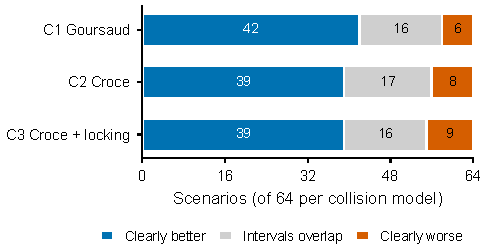
\includegraphics[width=\linewidth]{figs/fig_headroom.pdf}
\caption{\textbf{Knowing the Doppler limit helps under every collision model.} Scenarios in which the elevation-aware oracle delivers clearly more, comparably, or clearly less than link-only, out of 64 per collision model (seeds 21--25; ``clearly'' means non-overlapping 95\% intervals).}
\label{fig:headroom}
\end{figure}

\subsection{Controller Performance}
The controller lowered delivery in none of the 192 scenarios. It sets a cut-off only at low latitude with 5~dBi, where SF12 is used at high elevation. At mid-latitude with 5~dBi, SF12 is received only between 20$^\circ$ and 30$^\circ$, and at 10~dBi the cut-off is not triggered either; there it stays at 90$^\circ$ and the controller matches link-only exactly.

Where Doppler loss occurs, the controller learns quickly. In the C3, R1, 500-device scenario, all five seeds run pass~0 without a cut-off, three set one after pass~1, and all hold 50$^\circ$ from pass~2 on (Fig.~\ref{fig:doppler}c). The Doppler-loss share falls from 13.4\% on pass~0 to between 7.5\% and 12\% afterwards.

Across R1, R2 and R4 at low latitude and 5~dBi, the Doppler-loss share is clearly lower in 24 of the 34 scenarios with Doppler loss (Fig.~\ref{fig:doppler}a,~b), for example from 13.0\% to 11.2\% in C3, R1 with 100 devices. In the other ten the mean is lower but the intervals overlap; these are mostly 5000-device scenarios, where collisions dominate, and R2 with 100 devices. Elsewhere, residual Doppler losses of up to 18\% come from SF10 under the analytical limit and disappear under R4, so an SF12 cut-off cannot address them.

\begin{figure*}[t]
\centering
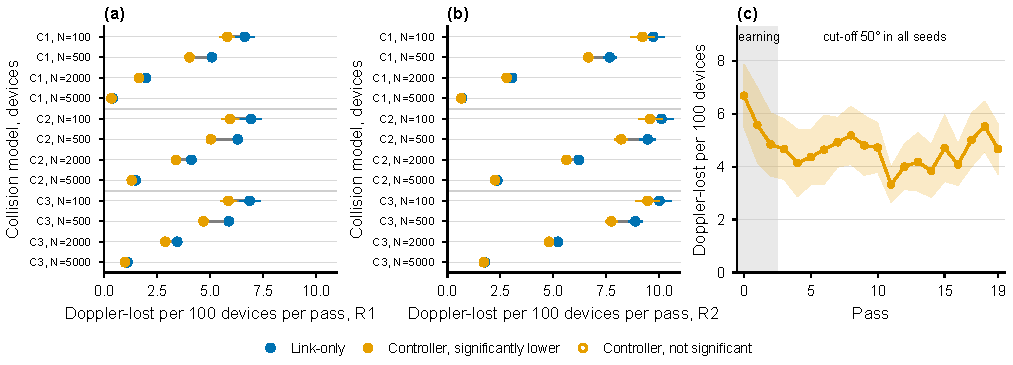
\includegraphics[width=\linewidth]{figs/fig_doppler.pdf}
\caption{\textbf{The controller lowers Doppler loss at low latitude and learns its cut-off within two passes.} (a, b) Doppler-loss share of link-only and the controller at low latitude and 5~dBi under R1 and R2; mean of 10 seeds with 95\% intervals; open markers overlap link-only. R4 equals R1 in this setting and is omitted; C1 with 5000 devices under R1 was outside the test scope. (c) Doppler-loss share per pass for C3, R1, 500 devices; mean of 5 seeds, band is the 95\% interval; shading marks the passes before all seeds hold 50$^\circ$.}
\label{fig:doppler}
\end{figure*}

\subsection{What Limits the Controller}
The oracle still delivers more (Table~\ref{tab:c3}): at low latitude with 5~dBi the controller reaches 0.65 to 0.76 of oracle delivery under R1, R2 and R4, compared on the same seeds 21--25.

\begin{table}[t]
\centering
\caption{Delivery and Doppler loss under C3, low latitude, 5~dBi}\label{tab:c3}
\setlength{\tabcolsep}{4pt}
\begin{tabular}{@{}llccccc@{}}
\toprule
 & & \multicolumn{3}{c}{Packets per device per pass} & \multicolumn{2}{c}{Doppler loss (\%)} \\
\cmidrule(lr){3-5}\cmidrule(l){6-7}
 & $N$ & Link-only & Controller & Oracle & Link-only & Controller \\
\midrule
R1 & 100  & 0.075 & 0.079 & 0.103 & 13.0 & \textbf{11.2} \\
   & 500  & 0.070 & 0.075 & 0.098 & 11.2 & \textbf{9.0} \\
   & 2000 & 0.054 & 0.058 & 0.079 & 6.5 & \textbf{5.5} \\
   & 5000 & 0.034 & 0.037 & 0.049 & 2.1 & 1.9 \\
\midrule
R2 & 100  & 0.044 & 0.044 & 0.071 & 19.0 & 18.1 \\
   & 500  & 0.040 & 0.045 & 0.069 & 16.8 & \textbf{14.8} \\
   & 2000 & 0.036 & 0.039 & 0.060 & 9.9 & \textbf{9.2} \\
   & 5000 & 0.027 & 0.029 & 0.044 & 3.4 & 3.3 \\
\bottomrule
\end{tabular}
\\[2pt]
\parbox{\linewidth}{\footnotesize Link-only and controller: means of seeds 21--30; oracle: seeds 21--25. Bold: clearly lower than link-only (non-overlapping 95\% intervals). R4 is identical to R1 here.}
\end{table} Two causes are plausible. Only 43\% of devices hear a beacon at low latitude, so most devices may never learn the cut-off; or one elevation threshold may be too coarse.

We tested the first cause directly by applying the controller's settings to every device at each pass boundary, with beacons off. With criteria fixed in advance, instant delivery would count as the limit if it was clearly better in at least 27 of the 36 low-latitude 5~dBi scenarios. It was clearly better in none, and closed a median of 1\% of the gap to the oracle (range $-3\%$ to 20\%; Fig.~\ref{fig:limit}). At 10~dBi, where no cut-off is learned, it changed no scenario, as expected.

The remaining gap comes from the threshold itself. The Doppler rate a device sees at a given elevation depends on how close the pass comes to zenith. Over the pass geometries in our runs, any single elevation threshold misclassifies 13.3\% of SF12 decisions under R1 and 30.0\% under R2: it either withholds SF12 from packets that would survive or allows it for packets that will not. Closing the gap needs a rule on Doppler rate, which a device could compute from published ephemeris and its own position.

Such a rule moves work to the device. A static sensor knows its position once; it would also need recent orbital elements, which trajectory-based policies already assume~\cite{alvarez2022}, and the time, which Class~B beacons carry~\cite{lorawanL2}. With these, the device can evaluate \eqref{eq:doppler} over the time on air of each candidate packet and withhold SF12 only when the predicted rate exceeds the limit. The network would then only have to estimate that limit, and the gateway's counts by elevation could serve that purpose. We leave this split design to future work.

A learning controller does not fix this from network data alone. A contextual bandit that chose a Doppler-rate threshold per pass did no harm but performed worse than the elevation rule in all 36 target scenarios, because the reward differences between thresholds (a few packets per pass) were far smaller than the variation between passes.

\begin{figure*}[t]
\centering
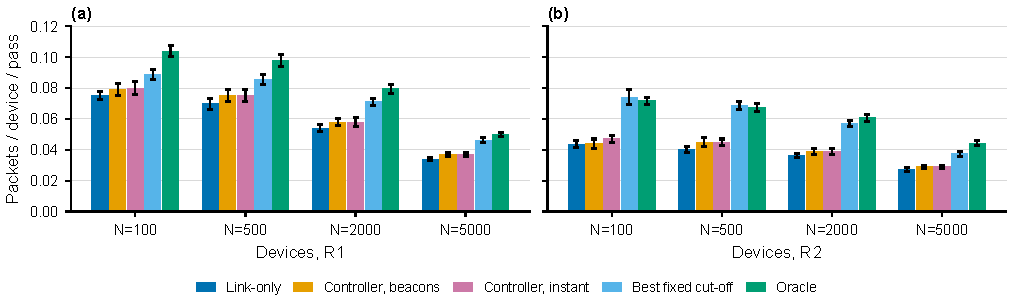
\includegraphics[width=\linewidth]{figs/fig_limit.pdf}
\caption{\textbf{Instant delivery of settings gains nothing over beacons; the gap to the oracle remains.} Delivered packets per device per pass for C3 at low latitude and 5~dBi under (a) R1 and (b) R2. Link-only and both controller variants: 10 seeds; oracle: 5 seeds; whiskers are 95\% intervals.}
\label{fig:limit}
\end{figure*}

\subsection{Negative Result: Load Control}
The network also sees how many devices it hears, which suggests thinning the offered load with a broadcast transmit probability~\cite{vogelgesang2021,alvarez2022}. With the true number of devices known, a fixed probability lowered airtime per delivered packet without clearly lowering delivery in 11 of 16 high-load scenarios under C1, but in only 5 of 16 under C2 and 7 of 16 under C3. Rules that estimated the load from gateway counts did worse: $p=k/\hat n$ cut delivery to 0.15--0.22 of link-only in its worst tuning scenario, and every threshold of a two-level rule cost at least 13\% of delivery somewhere. The only regime in which thinning helped under all three collision models was mid-latitude, 5~dBi and 5000 devices, where airtime per delivered packet fell to 0.29--0.56 of link-only. In this setting, whether load control pays off depends on the collision model, and gateway counters were too coarse to apply it without harm.

\section{Discussion and Limitations}\label{sec:discussion}
\emph{Unmeasured limits.} The size of every Doppler result depends on the SF12 limit at 868~MHz. Under R3 there is no loss to remove, and the controller sets no cut-off. A measurement of SF12 and SF10 Doppler-rate tolerance at 868~MHz on a gateway-class receiver would settle which reading applies.

\emph{Gateway receiver.} C2 and C3 come from single-receiver SX1272 measurements~\cite{croce2018,bor2016}. A satellite gateway would use a multi-demodulator chip such as the SX1301~\cite{sx1301}, for which no capture measurement is available.

\emph{Other simplifications.} The beacon power is the terrestrial short-range limit, assumed for the satellite. Device oscillator offset is not modeled; a few kilohertz at 868~MHz could matter near the SF12 static limit. Per-pass control runs on the non-real-time timescale of O-RAN rApps~\cite{tarchi2026}, not the near-real-time timescale of xApps. All results come from simulation.

\section{Conclusion}
The network can see SF12 Doppler loss in its own reception counts and act on it. A per-pass controller that learns one elevation cut-off and sends it in Class~B beacons never harmed delivery across 192 scenarios and clearly reduced Doppler loss in 24 of the 34 where it occurs. Its gain is capped by the coarseness of a single elevation threshold, and faster delivery of settings did not raise it. Thinning load from gateway counters did not survive measured collision thresholds. Future work should measure the SF12 Doppler-rate limit at 868~MHz and test device-side Doppler-rate rules driven by ephemeris.

\section*{Acknowledgment}
The author used Claude (Anthropic) as an AI assistant during this work. It helped write the simulation and analysis code, produce the figures from the simulation data, organize the literature search, and draft and edit the text of all sections. The author chose the research questions and the experiment design, supplied and checked all cited sources, reviewed every result against the simulation logs, and revised the final text. The author takes full responsibility for the content of this article.

\begin{thebibliography}{99}

\bibitem{alvarez2022} G.~\'Alvarez, J.~A. Fraire, K.~A. Hassan, S.~C\'espedes, and D.~Pesch, ``Uplink transmission policies for LoRa-based direct-to-satellite IoT,'' \emph{IEEE Access}, vol.~10, pp.~72687--72701, 2022, doi:10.1109/ACCESS.2022.3189647.

\bibitem{asadullah2024} M.~Asad~Ullah, G.~Pasolini, K.~Mikhaylov, and H.~Alves, ``Understanding the limits of LoRa direct-to-satellite: The Doppler perspectives,'' \emph{IEEE Open J. Commun. Soc.}, vol.~5, pp.~51--63, 2024, doi:10.1109/OJCOMS.2023.3337004.

\bibitem{zadorozhny2022} A.~M. Zadorozhny, A.~A. Doroshkin, V.~N. Gorev, A.~V. Melkov, A.~A. Mitrokhin, V.~Yu. Prokopyev, and Y.~M. Prokopyev, ``First flight-testing of LoRa modulation in satellite radio communications in low-Earth orbit,'' \emph{IEEE Access}, vol.~10, pp.~100006--100023, 2022, doi:10.1109/ACCESS.2022.3207762.

\bibitem{doroshkin2019} A.~A. Doroshkin, A.~M. Zadorozhny, O.~N. Kus, V.~Yu. Prokopyev, and Y.~M. Prokopyev, ``Experimental study of LoRa modulation immunity to Doppler effect in CubeSat radio communications,'' \emph{IEEE Access}, vol.~7, pp.~75721--75731, 2019, doi:10.1109/ACCESS.2019.2919274.

\bibitem{colombo2022} R.~M. Colombo, A.~Mahmood, E.~Sisinni, P.~Ferrari, and M.~Gidlund, ``Low-cost SDR-based tool for evaluating LoRa satellite communications,'' in \emph{Proc. IEEE Int. Symp. Measurements \& Networking (M\&N)}, 2022, doi:10.1109/MN55117.2022.9887761.

\bibitem{sx1301} Semtech, \emph{SX1301 Datasheet}, rev.~2.4.

\bibitem{sx1276} Semtech, \emph{SX1276/77/78/79 Datasheet}.

\bibitem{tarchi2026} D.~Tarchi, ``AI lifecycle-aware feasibility framework for split-RIC orchestration in NTN O-RAN,'' arXiv:2603.23252, 2026.

\bibitem{lorawanL2} LoRa Alliance, \emph{LoRaWAN L2 1.0.4 Specification}, 2020.

\bibitem{lorawanRP} LoRa Alliance, \emph{LoRaWAN Regional Parameters v1.0.2}, 2017.

\bibitem{goursaud2015} C.~Goursaud and J.-M. Gorce, ``Dedicated networks for IoT: PHY/MAC state of the art and challenges,'' \emph{EAI Endorsed Trans. Internet of Things}, 2015, doi:10.4108/eai.26-10-2015.150597.

\bibitem{croce2018} D.~Croce, M.~Gucciardo, S.~Mangione, G.~Santaromita, and I.~Tinnirello, ``Impact of LoRa imperfect orthogonality: Analysis of link-level performance,'' \emph{IEEE Commun. Lett.}, vol.~22, no.~4, pp.~796--799, 2018.

\bibitem{bor2016} M.~C. Bor, U.~Roedig, T.~Voigt, and J.~M. Alonso, ``Do LoRa low-power wide-area networks scale?'' in \emph{Proc. ACM MSWiM}, 2016, pp.~59--67.

\bibitem{rahmadhani2018} A.~Rahmadhani and F.~Kuipers, ``When LoRaWAN frames collide,'' in \emph{Proc. ACM WiNTECH}, 2018, pp.~89--97, doi:10.1145/3267204.3267212.

\bibitem{tondo2024} F.~A. Tondo, M.~Afhamisis, S.~Montejo-S\'anchez, O.~L. Alcaraz~L\'opez, M.~R. Palattella, and R.~D. Souza, ``Multiple channel LoRa-to-LEO scheduling for direct-to-satellite IoT,'' \emph{IEEE Access}, vol.~12, pp.~30627--30637, 2024, doi:10.1109/ACCESS.2024.3368872.

\bibitem{maleki2026} A.~Maleki, E.~Bedeer, and R.~Barton, ``Packet loss analysis under Doppler effects and reinforcement-learning-based resource allocation for direct-to-satellite LoRaWAN,'' arXiv:2610.23682, 2026.

\bibitem{herreria2023} S.~Herrer\'ia-Alonso, M.~Rodr\'iguez-P\'erez, R.~F. Rodr\'iguez-Rubio, and F.~P\'erez-Font\'an, ``Improving uplink scalability of LoRa-based direct-to-satellite IoT networks,'' \emph{IEEE Internet Things J.}, vol.~11, no.~7, pp.~12526--12535, 2024, doi:10.1109/JIOT.2023.3333934.

\bibitem{vogelgesang2021} K.~Vogelgesang, J.~A. Fraire, and H.~Hermanns, ``Uplink transmission probability functions for LoRa-based direct-to-satellite IoT: A case study,'' in \emph{Proc. IEEE GLOBECOM}, 2021, doi:10.1109/GLOBECOM46510.2021.9685152.

\bibitem{fsma2026} R.~R. Vennam, M.~Zhang, R.~Subbaraman, D.~Vasisht \emph{et al.}, ``FSMA: Gateway-controlled access for scalable LoRa non-terrestrial networks,'' in \emph{Proc. ACM MobiHoc}, 2026, arXiv:2510.02800.

\bibitem{traspadini2025} A.~Traspadini, M.~Zorzi, and M.~Giordani, ``Performance evaluation of LoRa for IoT applications in non-terrestrial networks via ns-3,'' arXiv:2509.02811, 2025.

\bibitem{casals2017} L.~Casals, B.~Mir, R.~Vidal, and C.~Gomez, ``Modeling the energy performance of LoRaWAN,'' \emph{Sensors}, vol.~17, no.~10, art.~2364, 2017, doi:10.3390/s17102364.

\bibitem{tr38811} 3GPP, ``Study on New Radio (NR) to support non-terrestrial networks,'' TR 38.811, V15.1.0.

\bibitem{santana2026} J.~M. de~Souza~Sant'Ana, N.~H. Mahmood, and V.~P. Borin, ``Performance analysis of LoRa and LR-FHSS in 3GPP LEO satellite and HAPS channel scenarios for remote area IoT coverage,'' arXiv:2609.07291, 2026.

\bibitem{erc7003} CEPT, ``ERC Recommendation 70-03 relating to the use of short range devices,'' Feb. 2022.

\bibitem{ns3lorawan} SIGNET Lab, University of Padova, ``LoRaWAN module for ns-3,'' \url{https://github.com/signetlabdei/lorawan}, commit e45b4af.

\end{thebibliography}

\begin{IEEEbiography}[{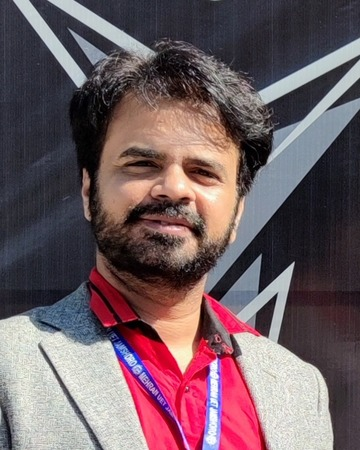
\includegraphics[width=1in,height=1.25in,clip,keepaspectratio]{figs/author_photo.jpg}}]{Mehran M. Mamonai}
received the B.E. degree in telecommunication engineering from Mehran University of Engineering and Technology (MUET), Jamshoro, Pakistan, in 2009, and the M.E. degree in electronics and telecommunication engineering from Universiti Teknologi Malaysia (UTM), Johor Bahru, Malaysia, in 2015. He is currently pursuing the Ph.D. degree in telecommunication engineering with MUET, where he is an Assistant Professor and the Final Year Project--Industry Focal Person with the Department of Telecommunication Engineering. He is also a cybersecurity trainer for the Pakistan Information Technology Program, Government of Sindh. His research interests include wireless communications, IoT architectures, LoRaWAN, Open RAN, embedded systems, cybersecurity, and antenna fabrication.
\end{IEEEbiography}

\end{document}
